\documentclass[twocolumn, a4j]{jsarticle}

\usepackage{listings, jlisting, color}
\usepackage[dvipdfmx]{graphicx}
\usepackage{pdfpages}
\usepackage{amsmath}
\usepackage{mathtools}
\usepackage{multirow}
\usepackage{color}
\usepackage{ulem}
\usepackage{here}
\usepackage{wrapfig}
\usepackage[margin=20mm]{geometry}
%%図を二個横に並べるときに使用
\usepackage[hang,small,bf]{caption}
\usepackage[subrefformat=parens]{subcaption}
%%\urlを使用する際に必要
\usepackage{url}

\renewcommand{\baselinestretch}{0.78}

\setlength{\columnwidth}{5mm}

\lstset{
  basicstyle={\ttfamily},
  identifierstyle={\small},
  commentstyle={\smallitshape},
  keywordstyle={\small\bfseries},
  ndkeywordstyle={\small},
  stringstyle={\small\ttfamily},
  frame={tb},
  breaklines=true,
  columns=[l]{fullflexible},
  numbers=left,
  xrightmargin=0zw,
  xleftmargin=3zw,
  numberstyle={\scriptsize},
  stepnumber=1,
  numbersep=1zw,
  lineskip=-0.5ex
}

\makeatletter % プリアンブルで定義開始

% 表示文字列を"図"から"Figure”へ,"表"から"Table”へ
\renewcommand{\figurename}{図}
\renewcommand{\tablename}{表}

% 図,表番号を"<章番号>.<図番号>” ,"<章番号>.<表番号>” へ
\renewcommand{\thefigure}{\thesection-\arabic{figure}}
\renewcommand{\thetable}{\thesection-\arabic{table}}

% 章が進むごとに図番号をリセットする
\@addtoreset{figure}{section}
\@addtoreset{table}{section}

\makeatother % プリアンブルで定義終了

\begin{document}
\twocolumn[
  \title{
    LSIデザインコンテスト 進捗報告
    \large{\\---画像をVAEで圧縮したい---}}
  \author{222C1021 今村優希}
  \maketitle

  \section{進捗概要}

]

\section{前回の振り返り}
前回は道路の画像を実際にVAEに通してみて,出力結果がどの様になるかの実験を行った.


\section{今回の実施内容}
使用したプログラムは前回でまとめたプログラムである.
\begin{itemize}
  \item 今まで作成したプログラムを一つにまとめたもの
  \begin{itemize}
    \item VAEの学習のみを行うプログラム
    \item VAEの学習済みの値を利用するプログラム
  \end{itemize}
\end{itemize}

また,システム構造の概略を作成した.

\section{実験と考察}
\subsection{実験1}
\subsubsection{内容}
「道路のみを学中させるVAE」で作成したプログラムを活用して実験を行う.
学習させる画像を図\ref{fig:4-1}に示す.
テストさせる画像を以下の図と図に設定する.
今回は,プログラム内部でグレースケール化をしてくれるので,カラー画像を挿入する.
\\条件:Layer2 = 16, epoch = 80,000, eta = 0.0005
\begin{figure}[h]
  \begin{center}
    \includegraphics[width=0.48\columnwidth]{figure/output_test11.bmp}
  \end{center}
  \caption{学習させた画像}
  \label{fig:4-1}
\end{figure}

\begin{figure}[h]
  \begin{minipage}[]{0.49\columnwidth}
    \centering
    \includegraphics[width=0.9\columnwidth]{figure/road_image2.bmp}
    \subcaption{学習率の推移}
    \label{fig:4-3-1}
  \end{minipage}
  \begin{minipage}[]{0.49\linewidth}
    \centering
    \includegraphics[width=0.9\columnwidth]{figure/road_image4.png}
    \subcaption{ブロックごとのPSNR\\ 黄色に近い色がPSNRが高い}
    \label{fig:4-3-2}
  \end{minipage}
  \caption{入力したブロック画像の出力結果}
  \label{fig:4-3}
\end{figure}

\subsubsection{結果}
VAEで学習し,教師データと同じ図\ref{fig:4-1}をテストデータとしてVAEに通過させた.
VAEからの出力画像と学習率の推移を図\ref{fig:4-2}に示す.
この画像におけるPSNRは31.146[dB]と,許容範囲内であった.
また,学習率及び,ブロックごとのPSNRのを測定したものを図に示す.
ブロックごとのPSNRに関して,黒い部分はPSNR=50として図に示している.
\begin{figure}[h]
  \begin{center}
    \includegraphics[width=0.9\columnwidth]{figure/output_test11.bmp}
  \end{center}
  \caption{テストデータの出力結果}
  \label{fig:4-2}
\end{figure}

\begin{figure}[h]
  \begin{minipage}[]{0.49\columnwidth}
    \centering
    \includegraphics[width=0.9\columnwidth]{figure/archive_20241224_resul11-2.png}
    \subcaption{学習率の推移}
    \label{fig:4-3-1}
  \end{minipage}
  \begin{minipage}[]{0.49\linewidth}
    \centering
    \includegraphics[width=0.9\columnwidth]{figure/untitled1.png}
    \subcaption{ブロックごとのPSNR\\ 黄色に近い色がPSNRが高い}
    \label{fig:4-3-2}
  \end{minipage}
  \caption{入力したブロック画像の出力結果}
  \label{fig:4-3}
\end{figure}

\subsubsection{考察}
道路中央部分はPSNRが高いが,道路の端の部分(道路ではない部分の近く)に関してはPSNRが低下している.
そもそも,端っこに対応するブロック数が少なく,VAEが過学習をしてしまったせいであると考察できる.

\subsection{実験2}
\subsubsection{内容}
前回の考察より,4隅に黒い部分がないブロックに関してだけ学習を行い,VAEに適切な学習を行うようVAEの学習アルゴリズムを変更した.
今回の内容では,今まで作成したプログラムを一つにまとめたプログラムを作成し,それを用いて実験を行った.
学習させる画像は実験1と同じものであるが,テストデータとしては様々な画像で試してみた.
\\条件:Layer2 = 32, epoch = 10,000, eta = 0.0001
\subsubsection{結果}
テストデータ毎に,入力,出力,ブロックごとのPSNRを出力させたものを示す.

\paragraph{結果1}
入力画像として図\ref{fig:4-4-1},出力画像が図\ref{fig:4-4-2}である.
また,PSNRは図\ref{fig:4-5}である.
\begin{figure}[h]
  \begin{minipage}[]{0.49\columnwidth}
    \centering
    \includegraphics[width=0.9\columnwidth]{figure/road_image2.bmp}
    \subcaption{入力画像}
    \label{fig:4-4-1}
  \end{minipage}
  \begin{minipage}[]{0.49\linewidth}
    \centering
    \includegraphics[width=0.9\columnwidth]{figure/output_test2.bmp}
    \subcaption{出力画像}
    \label{fig:4-4-2}
  \end{minipage}
  \caption{VAEの入出力結果}
  \label{fig:4-4}
\end{figure}
\begin{figure}[h]
  \begin{center}
    \includegraphics[width=0.9\columnwidth]{figure/archive_20241225_psnr2.png}
  \end{center}
  \caption{ブロックごとのPSNR}
  \label{fig:4-5}
\end{figure}

\paragraph{結果2}
入力画像として図\ref{fig:4-4-1},出力画像が図\ref{fig:4-4-2}である.
また,PSNRは図\ref{fig:4-5}である.
\begin{figure}[h]
  \begin{minipage}[]{0.49\columnwidth}
    \centering
    \includegraphics[width=0.9\columnwidth]{figure/road_image4.png}
    \subcaption{入力画像}
    \label{fig:4-6-1}
  \end{minipage}
  \begin{minipage}[]{0.49\linewidth}
    \centering
    \includegraphics[width=0.9\columnwidth]{figure/output_test4.bmp}
    \subcaption{出力画像}
    \label{fig:4-6-2}
  \end{minipage}
  \caption{VAEの入出力結果}
  \label{fig:4-7}
\end{figure}
\begin{figure}[h]
  \begin{center}
    \includegraphics[width=0.9\columnwidth]{figure/archive_20241225_psnr4.png}
  \end{center}
  \caption{ブロックごとのPSNR}
  \label{fig:4-8}
\end{figure}


\subsubsection{考察}
これらの結果から,道路の部分は評価の高いPSNRを出すことができている.
また,道路以外の部分に関してはPSNRが悪いためそれ用のアルゴリズムの考案が必要であると考えられる.
結果2より異常検知もうまくできているようなので,これからのシステム開発に応用できそうであると思う.

\section{課題}
\begin{itemize}
  \item 課題1\\
  低PSNRのブロックに対しての動作\\
  現在は,元の画像を持ってくるという対応を考えている.
  \item 課題2\\
  画像に応じてVAEが再学習するようなアルゴリズム考案
  \item 課題3\\
  ハードウェアの設計準備
  \end{itemize}

\section{今後の計画}
画像処理のシミュレーションはある程度できたので,ハードウェアの設計に取り組もうと考えている.
それと並行で,以上部分(PSNRの値が低い部分)の処理のシミュレーションも行おうと思っている.
また,課題3の実現可能性についても実験していきたいと思っている.
\begin{itemize}
  \item[1] ハードウェアの設計
  \item[2] アルゴリズム考案
  \item[3] 課題3の実現可能性の検討
\end{itemize}

\begin{figure}
  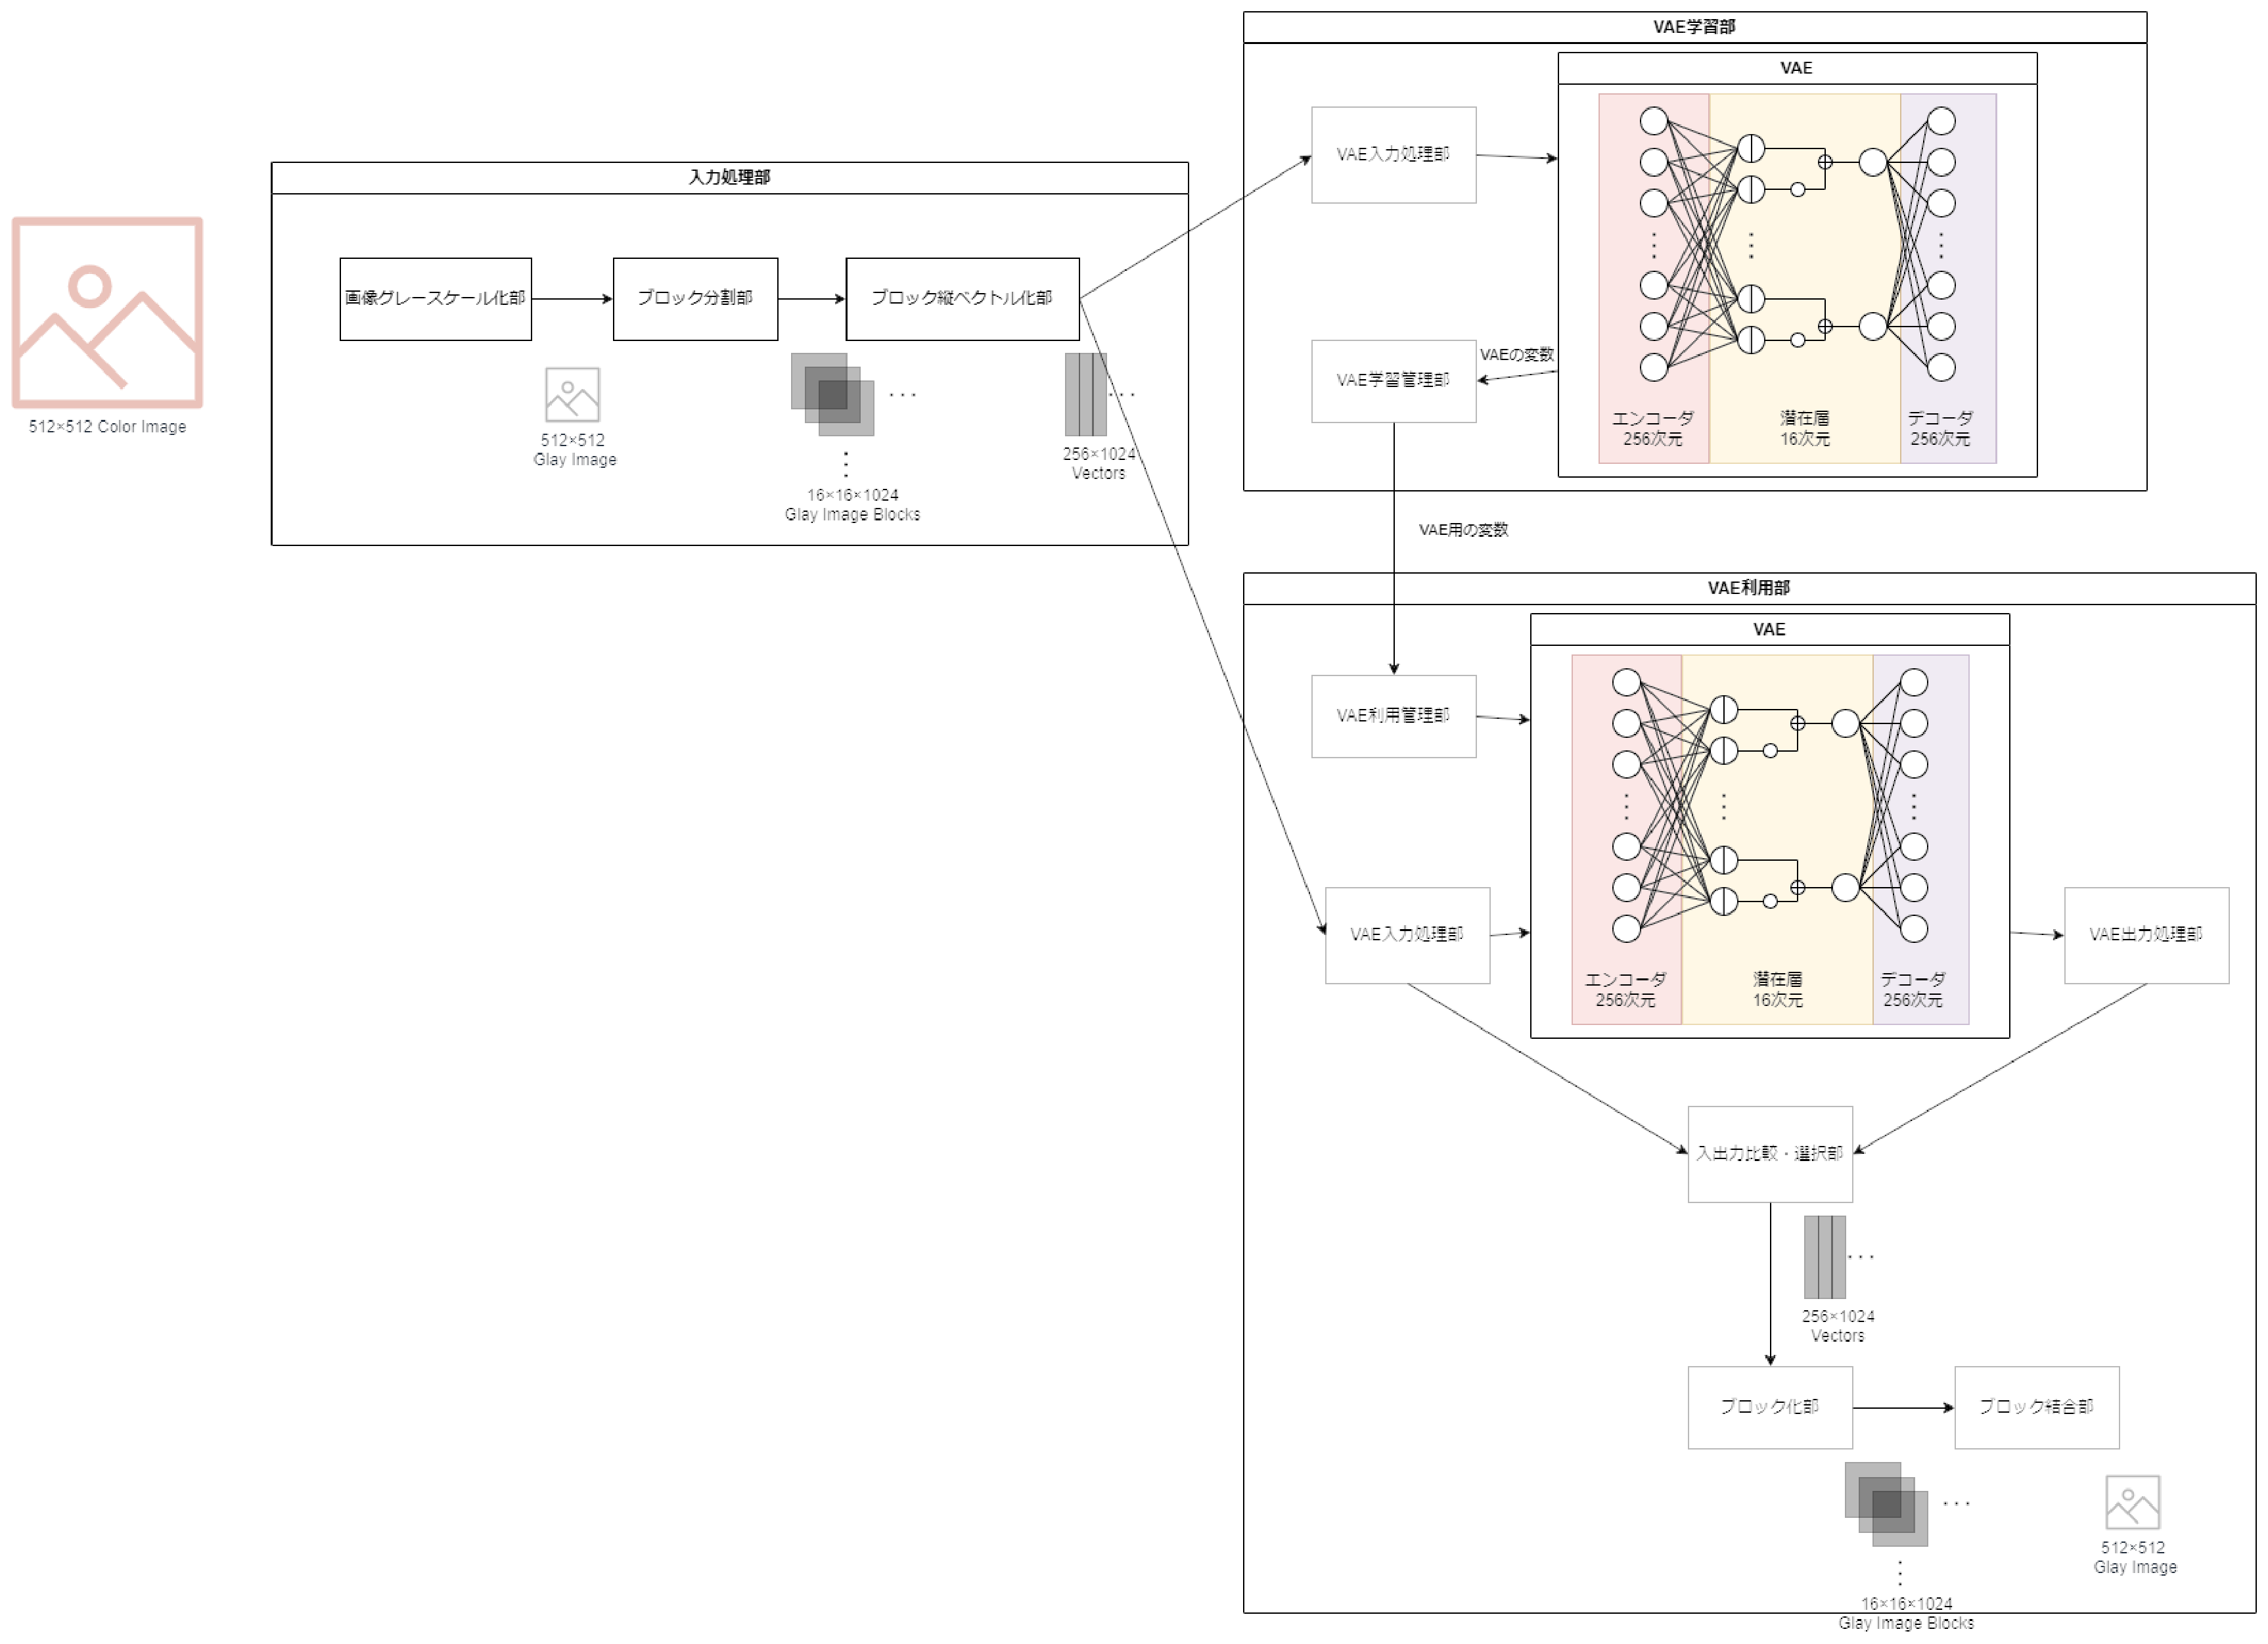
\includegraphics[scale=0.5]{figure/test.eps}
\end{figure}



\end{document}